\documentclass{ximera}
 

\usepackage{epsfig}

\graphicspath{
  {./}
  {figures/}
}

\usepackage{morewrites}
\makeatletter
\newcommand\subfile[1]{%
\renewcommand{\input}[1]{}%
\begingroup\skip@preamble\otherinput{#1}\endgroup\par\vspace{\topsep}
\let\input\otherinput}
\makeatother

\newcommand{\includeexercises}{\directlua{dofile("/home/jim/linearAlgebra/laode/exercises.lua")}}

%\newcounter{ccounter}
%\setcounter{ccounter}{1}
%\newcommand{\Chapter}[1]{\setcounter{chapter}{\arabic{ccounter}}\chapter{#1}\addtocounter{ccounter}{1}}

%\newcommand{\section}[1]{\section{#1}\setcounter{thm}{0}\setcounter{equation}{0}}

%\renewcommand{\theequation}{\arabic{chapter}.\arabic{section}.\arabic{equation}}
%\renewcommand{\thefigure}{\arabic{chapter}.\arabic{figure}}
%\renewcommand{\thetable}{\arabic{chapter}.\arabic{table}}

%\newcommand{\Sec}[2]{\section{#1}\markright{\arabic{ccounter}.\arabic{section}.#2}\setcounter{equation}{0}\setcounter{thm}{0}\setcounter{figure}{0}}

\newcommand{\Sec}[2]{\section{#1}}

\setcounter{secnumdepth}{2}
%\setcounter{secnumdepth}{1} 

%\newcounter{THM}
%\renewcommand{\theTHM}{\arabic{chapter}.\arabic{section}}

\newcommand{\trademark}{{R\!\!\!\!\!\bigcirc}}
%\newtheorem{exercise}{}

\newcommand{\dfield}{{\sf dfield9}}
\newcommand{\pplane}{{\sf pplane9}}

\newcommand{\EXER}{\section*{Exercises}}%\vspace*{0.2in}\hrule\small\setcounter{exercise}{0}}
\newcommand{\CEXER}{}%\vspace{0.08in}\begin{center}Computer Exercises\end{center}}
\newcommand{\TEXER}{} %\vspace{0.08in}\begin{center}Hand Exercises\end{center}}
\newcommand{\AEXER}{} %\vspace{0.08in}\begin{center}Hand Exercises\end{center}}

% BADBAD: \newcommand{\Bbb}{\bf}

\newcommand{\R}{\mbox{$\Bbb{R}$}}
\newcommand{\C}{\mbox{$\Bbb{C}$}}
\newcommand{\Z}{\mbox{$\Bbb{Z}$}}
\newcommand{\N}{\mbox{$\Bbb{N}$}}
\newcommand{\D}{\mbox{{\bf D}}}
\usepackage{amssymb}
%\newcommand{\qed}{\hfill\mbox{\raggedright$\square$} \vspace{1ex}}
%\newcommand{\proof}{\noindent {\bf Proof:} \hspace{0.1in}}

\newcommand{\setmin}{\;\mbox{--}\;}
\newcommand{\Matlab}{{M\small{AT\-LAB}} }
\newcommand{\Matlabp}{{M\small{AT\-LAB}}}
\newcommand{\computer}{\Matlab Instructions}
\newcommand{\half}{\mbox{$\frac{1}{2}$}}
\newcommand{\compose}{\raisebox{.15ex}{\mbox{{\scriptsize$\circ$}}}}
\newcommand{\AND}{\quad\mbox{and}\quad}
\newcommand{\vect}[2]{\left(\begin{array}{c} #1_1 \\ \vdots \\
 #1_{#2}\end{array}\right)}
\newcommand{\mattwo}[4]{\left(\begin{array}{rr} #1 & #2\\ #3
&#4\end{array}\right)}
\newcommand{\mattwoc}[4]{\left(\begin{array}{cc} #1 & #2\\ #3
&#4\end{array}\right)}
\newcommand{\vectwo}[2]{\left(\begin{array}{r} #1 \\ #2\end{array}\right)}
\newcommand{\vectwoc}[2]{\left(\begin{array}{c} #1 \\ #2\end{array}\right)}

\newcommand{\ignore}[1]{}


\newcommand{\inv}{^{-1}}
\newcommand{\CC}{{\cal C}}
\newcommand{\CCone}{\CC^1}
\newcommand{\Span}{{\rm span}}
\newcommand{\rank}{{\rm rank}}
\newcommand{\trace}{{\rm tr}}
\newcommand{\RE}{{\rm Re}}
\newcommand{\IM}{{\rm Im}}
\newcommand{\nulls}{{\rm null\;space}}

\newcommand{\dps}{\displaystyle}
\newcommand{\arraystart}{\renewcommand{\arraystretch}{1.8}}
\newcommand{\arrayfinish}{\renewcommand{\arraystretch}{1.2}}
\newcommand{\Start}[1]{\vspace{0.08in}\noindent {\bf Section~\ref{#1}}}
\newcommand{\exer}[1]{\noindent {\bf \ref{#1}}}
\newcommand{\ans}{}
\newcommand{\matthree}[9]{\left(\begin{array}{rrr} #1 & #2 & #3 \\ #4 & #5 & #6
\\ #7 & #8 & #9\end{array}\right)}
\newcommand{\cvectwo}[2]{\left(\begin{array}{c} #1 \\ #2\end{array}\right)}
\newcommand{\cmatthree}[9]{\left(\begin{array}{ccc} #1 & #2 & #3 \\ #4 & #5 &
#6 \\ #7 & #8 & #9\end{array}\right)}
\newcommand{\vecthree}[3]{\left(\begin{array}{r} #1 \\ #2 \\
#3\end{array}\right)}
\newcommand{\cvecthree}[3]{\left(\begin{array}{c} #1 \\ #2 \\
#3\end{array}\right)}
\newcommand{\cmattwo}[4]{\left(\begin{array}{cc} #1 & #2\\ #3
&#4\end{array}\right)}

\newcommand{\Matrix}[1]{\ensuremath{\left(\begin{array}{rrrrrrrrrrrrrrrrrr} #1 \end{array}\right)}}

\newcommand{\Matrixc}[1]{\ensuremath{\left(\begin{array}{cccccccccccc} #1 \end{array}\right)}}



\renewcommand{\labelenumi}{\theenumi)}
\newenvironment{enumeratea}%
{\begingroup
 \renewcommand{\theenumi}{\alph{enumi}}
 \renewcommand{\labelenumi}{(\theenumi)}
 \begin{enumerate}}
 {\end{enumerate}\endgroup}



\newcounter{help}
\renewcommand{\thehelp}{\thesection.\arabic{equation}}

%\newenvironment{equation*}%
%{\renewcommand\endequation{\eqno (\theequation)* $$}%
%   \begin{equation}}%
%   {\end{equation}\renewcommand\endequation{\eqno \@eqnnum
%$$\global\@ignoretrue}}

%\input{psfig.tex}

\author{Martin Golubitsky and Michael Dellnitz}

%\newenvironment{matlabEquation}%
%{\renewcommand\endequation{\eqno (\theequation*) $$}%
%   \begin{equation}}%
%   {\end{equation}\renewcommand\endequation{\eqno \@eqnnum
% $$\global\@ignoretrue}}

\newcommand{\soln}{\textbf{Solution:} }
\newcommand{\exercap}[1]{\centerline{Figure~\ref{#1}}}
\newcommand{\exercaptwo}[1]{\centerline{Figure~\ref{#1}a\hspace{2.1in}
Figure~\ref{#1}b}}
\newcommand{\exercapthree}[1]{\centerline{Figure~\ref{#1}a\hspace{1.2in}
Figure~\ref{#1}b\hspace{1.2in}Figure~\ref{#1}c}}
\newcommand{\para}{\hspace{0.4in}}

\renewenvironment{solution}{\suppress}{\endsuppress}

\ifxake
\newenvironment{matlabEquation}{\begin{equation}}{\end{equation}}
\else
\newenvironment{matlabEquation}%
{\let\oldtheequation\theequation\renewcommand{\theequation}{\oldtheequation*}\begin{equation}}%
  {\end{equation}\let\theequation\oldtheequation}
\fi

\makeatother

\begin{document}

\CEXER

\noindent In Exercises~\ref{c14.3.7a} -- \ref{c14.3.7d} use \Matlab
to find solutions for the electrical circuit\index{electrical circuit} 
\eqref{E:RCLMcir}.  In each exercise, set $R=0$ and $C=L=1$ in addition to 
the specified information, and use the first order system \eqref{E:ECsy}.

\begin{exercise} \label{c14.3.7a}
Parameters for the circuit: $R_{mic}(t) = 1+\cos(5t)$ and $V(t) = 1$;\\
initial conditions and time interval: $x(0) = 1$, $\dot{x}(0) = 0.9$ and  
$t\in[0,20]$.

\begin{solution}
\ans The numerically computed solution is displayed in 
Figure~\ref{c14.3.7a}.

\soln  Using the system \eqref{E:ECsy} derived in 
Exercise~\ref{c14.3.4A}, the first order system is:
\begin{eqnarray*}
\dot{x} & = & y \\
\dot{y} & = & -x - (1+\cos(5t))y + 1
\end{eqnarray*}
with initial conditions $x(0)=1$ and $y(0)=0.9$.   To solve this system numerically 
using {\tt ode45}, write the m-file
\begin{verbatim}
function f = ex17_4_6(t,x)
A = [0  1; -1  -(1+cos(5*t))];
f = A*x + [0; 1];
\end{verbatim}
Now solve the differential equation using the command
\begin{verbatim}
[t,x] = ode45('ex17_4_6',[0 20],[1;0.9]);
\end{verbatim}
The solution $x(t)$ may be plotted using the command {\tt plot(t,x(:,1))}; the 
result is displayed in Figure~\ref{c14.3.7a}.
\begin{figure}[htb]
     \centerline{%
     \psfig{file=exfigure/fig17-4-6.eps,width=3.0in}}
        \exercap{c14.3.7a}
\end{figure} 


\end{solution}
\end{exercise}

\begin{exercise} \label{c14.3.7b}
Parameters for the circuit: $R_{mic}(t) = 1+\sin t$ and $V(t) = \sin(2t)$;\\
initial conditions and time interval: $x(0) = 2$, $\dot{x}(0) = 1$ and $t\in[0,40]$.

\begin{solution}
\ans The numerically computed solution is displayed in 
Figure~\ref{c14.3.7b}.

\soln  Using the system \eqref{E:ECsy} derived in 
Exercise~\ref{c14.3.4A}, the first order system is:
\begin{eqnarray*}
\dot{x} & = & y \\
\dot{y} & = & -x - (1+\sin t)y + \sin(2t)
\end{eqnarray*}
with initial conditions $x(0)=2$ and $y(0)=1$.  To solve this system numerically 
using {\tt ode45}, write the m-file
\begin{verbatim}
function f = ex17_4_7(t,x)
A = [0  1; -1  -(1+sin(t))];
f = A*x + [0; sin(2*t)];
\end{verbatim}
Now solve the differential equation using the command
\begin{verbatim}
[t,x] = ode45('ex17_4_7',[0 40],[2;1]);
\end{verbatim}
The solution $x(t)$ may be plotted using the command {\tt plot(t,x(:,1))}; the 
result is displayed in Figure~\ref{c14.3.7b}.
\begin{figure}[htb]
     \centerline{%
     \psfig{file=exfigure/fig17-4-7.eps,width=3.0in}}
        \exercap{c14.3.7b}
\end{figure} 


\end{solution}
\end{exercise}

\begin{exercise} \label{c14.3.7c}
Parameters for the circuit: $R_{mic}(t) = 1+\cos t$ and $V(t) = 0.4+e^{-t}\sin(3t)$;\\
initial conditions and time interval: $x(0) = 1$, $\dot{x}(0) = -1.5$ and 
$t\in[0,30]$.

\begin{solution}
\ans The numerically computed solution is displayed in 
Figure~\ref{c14.3.7c}.

\soln  Using the system \eqref{E:ECsy} derived in 
Exercise~\ref{c14.3.4A}, the first order system is:
\begin{eqnarray*}
\dot{x} & = & y \\
\dot{y} & = & -x - (1+\cos t)y + 0.4 + e^{-t}\sin t
\end{eqnarray*}
with initial conditions $x(0)=1$ and $y(0)=-1.5$. To solve this system numerically 
using {\tt ode45}, write the m-file
\begin{verbatim}
function f = ex17_4_8(t,x)
A = [0  1; -1  -(1+cos(t))];
f = A*x + [0; 0.4+exp(-t)*sin(t)];
\end{verbatim}
Now solve the differential equation using the command
\begin{verbatim}
[t,x] = ode45('ex17_4_8',[0 30],[1;-1.5]);
\end{verbatim}
The solution $x(t)$ may be plotted using the command {\tt plot(t,x(:,1))}; the 
result is displayed in Figure~\ref{c14.3.7c}.
\begin{figure}[htb]
     \centerline{%
     \psfig{file=exfigure/fig17-4-8.eps,width=3.0in}}
        \exercap{c14.3.7c}
\end{figure} 



\end{solution}
\end{exercise}

\begin{exercise} \label{c14.3.7d}
Parameters for the circuit: $R_{mic}(t) = 0.02+\sin t$ and $V(t) = 1$;\\
initial conditions and time interval: $x(0) = 1.2$, $\dot{x}(0) = 1.1$ and 
$t\in[0,60]$.

\begin{solution}
\ans The numerically computed solution is displayed in 
Figure~\ref{c14.3.7d}.

\soln  Using the system \eqref{E:ECsy} derived in 
Exercise~\ref{c14.3.4A}, the first order system is:
\begin{eqnarray*}
\dot{x} & = & y \\
\dot{y} & = & -x - (0.02+\sin t)y + 1
\end{eqnarray*}
with initial conditions $x(0)=1.2$ and $y(0)=1.1$.   To solve this system numerically 
using {\tt ode45}, write the m-file
\begin{verbatim}
function f = ex17_4_9(t,x)
A = [0  1; -1  -(0.02+sin(t))];
f = A*x + [0; 1];
\end{verbatim}
Now solve the differential equation using the command
\begin{verbatim}
[t,x] = ode45('ex17_4_9',[0 60],[1.2;1.1]);
\end{verbatim}
The solution $x(t)$ may be plotted using the command {\tt plot(t,x(:,1))}; the 
result is displayed in Figure~\ref{c14.3.7d}.
\begin{figure}[htb]
     \centerline{%
     \psfig{file=exfigure/fig17-4-9.eps,width=3.0in}}
        \exercap{c14.3.7d}
\end{figure} 





\end{solution}
\end{exercise}
\end{document}
